%Variables
\def \authorOne {BALTODANO BELTRÁN, Massiel Estela}
\def \authorTwo {SIAPO RODRÍGUEZ, José Luis Octavio}
\def \assessor {PERALTA LUJÁN, José Luis}
\def \titleTesis {Obtención de rasgos de personalidad a partir de evaluación parcial del test de Machover en imágenes realizadas por alumnos mayores de 12 años}

%%%%%%%%%%%%%%%%%%%%%%%%%%%%% CARATULA%%%%%%%%%%%%%%%%%%%%%%%%
\textheight 19cm
\pagestyle{empty}
\begin{center}
 {\bf {\fontsize{14}{16.8}\selectfont UNIVERSIDAD NACIONAL DE TRUJILLO}}     
 
    {\bf{\fontsize{14}{16.8}\selectfont Facultad de Ciencias Físicas y Matemáticas}} 

  {\bf{\fontsize{14}{16.8}\selectfont Escuela Profesional de Informática}}
\end{center}  

\begin{figure}[ht]
\begin{center}

\includegraphics[width=.4\textwidth]{images/unt}
\end{center}
\end{figure}
\vskip 0.5cm

\begin{center}
  {\bf\Large{{\fontsize{17}{20.4}\selectfont{Modelo para la ruterización} }}}     
\end{center}
\vskip 0.5cm

\begin{center}
{\Large{TESIS}}
\end{center}
\begin{center}
{\large{\hspace*{0.4cm} PARA OPTAR EL TÍTULO PROFESIONAL DE INGENIERO  INFORMÁTICO}}
\end{center}

\vskip 0.6cm
\begin{center}
  { \fontsize{14}{16.8}\selectfont {\hspace{-2.9cm}AUTOR(ES): \authorone}} \\
    { \fontsize{14}{16.8}\selectfont {\hspace{-0.4cm} \authortwo}}\\
    \vskip 0.2cm
    { \fontsize{14}{16.8}\selectfont {\hspace{-1.7cm} ASESOR: Dr. Rodríguez Melquiades José A.}}

     
\end{center}   


\vskip 1.1cm
\begin{center}    
{\bf {\fontsize{14}{16.8}\selectfont TRUJILLO - PERÚ
\vskip 0.0cm
\hspace*{-0.2cm} 
2019 }}
\end{center} 
\newpage
%%%%%%%%%%%%%%%%%%%%%%%%%%%%%%%%%%%%%%%%%%%%%%%%%%%%%%%%%%%%%%%%%%%%%%%%%%%


%%%%%%%%%%%%%%%%%%%%%%%%%%%%CONTRA CARATULA 1 %%%%%%%%%%%%%%%%%%%%%%%%%%%%%
%\newpage
%\pagestyle{plain}
%\pagenumbering{roman}

%\hspace*{6cm}
%\vskip 9cm
%\begin{center}
%   {\bf \doublespacing {\fontsize{17}{20.4}\selectfont{MODELO PARA LA RUTERIZACIÓN }}}     
%\end{center} 
%\newpage
%%%%%%%%%%%%%%%%%%%%%%%%%%%%%%%%%%%%%%%%%%%%%%%%%%%%%%%%%%%%%%%%%%%%%%%%%%%


%%%%%%%%%%%%%%%%%%%%%%%%%%%%% CONTRA CARATULA 2 %%%%%%%%%%%%%%%%%%%%%%%
%\begin{center}
%   {\bf {\fontsize{14}{16.8}\selectfont{EDGAR PECHE PERLADO}}}\\    
%      {\bf {\fontsize{14}{16.8}\selectfont{MANUEL PEREZ YON}}}       
%   \end{center}   

%\vskip 3.2cm
%\begin{center}
%   {\bf \doublespacing {\fontsize{17}{20.4}\selectfont{MODELO PARA LA RUTERIZACIÓN }}}     
%\end{center}   
%  \vskip 2cm
%\begin{verse}
% \fontsize{12}{14.4}\selectfont{\hspace*{0.6cm}Tesis presentada a la Escuela Profesional de Informática en la Facultad de Ciencias Físicas y Matemáticas de la Universidad Nacional de Trujillo, como requisito parcial para la obtención del grado de Bachiller en ciencia de la computación ( Título profesional de Ing. Informático)}
%\end{verse}

%\vskip 1.5cm 
%{\fontsize{14}{16.8}\selectfont ASESOR: JOSÉ A. RODRIGUEZ MELQUIADES} 
% \vskip 1cm 
% \begin{center}    
% \vskip 2cm
%{\fontsize{14}{16.8}\selectfont Trujillo - Perú
%\vskip 0.2cm
%\hspace*{-0.2cm} 
%2019}
%\end{center} 
%\newpage
%%%%%%%%%%%%%%%%%%%%%%%%%%%%%%%%%%%%%%%%%%%%%%%%%%%%%%%%%%%%%%%%%%%


%%%%%%%%%%%%%%%%%%%%%%%%%%%% DEDICATORIA %%%%%%%%%%%%%%%%%%%%%%
\pagestyle{plain}
\pagenumbering{roman}
 
 \addcontentsline{toc}{chapter}{Dedicatoria}
 {\bf\Large {Dedico esta tesis a :}}
 \vskip 1cm
\begin{quotation}
{\it Mis padres ....
\vskip 1cm
Mi hermano ... .
\vskip 1cm
Mi ... .}
\end{quotation}
%%%%%%%%%%%%%%%%%%%%%%%%%%%%%%%%%%%%%%%%%%%%%%%%%%%%%%%%%%%%%%%%%%%%%%%%%%%


\newpage

 \addcontentsline{toc}{chapter}{Agradecimientos}
 {\bf\Large {\flushleft{Agradecimientos}}}
 \vskip 1.5cm
\begin{quotation}
Agradezco a Dios por haberme bendecido en toda mi vida ....
{\vskip 1cm}
A mis profesores del Departamento de Informática, de los cuales recibi una gran cantidad de conocimientos  . . .
\vskip 1cm
A mi asesor Prof. Dr. José A. Rodríguez Melquiades que siempre se mostro disponible e interesado en ayudarme.
\vskip 1cm
 . . .
 \end{quotation}
\newpage 
%%%%%%%%%%%%%%%%%%%%%%%%%%%%%%%%%%%%%%%%%%%%%%%%%%%%%%%%%%%%%%%%%%%%%%%%%%%
              % Datos de la tesis

%%%%%%%%%%%%%%%%%%%%%%%%%%%% AGRADECIMENTOS %%%%%%%%%%%%%%%%%%%%%%

%%%%%%%%%%%%%%%%%%%%   ACTA SUSTENTACION   %%%%%%%%%%%%%%%%%%%%%%%%

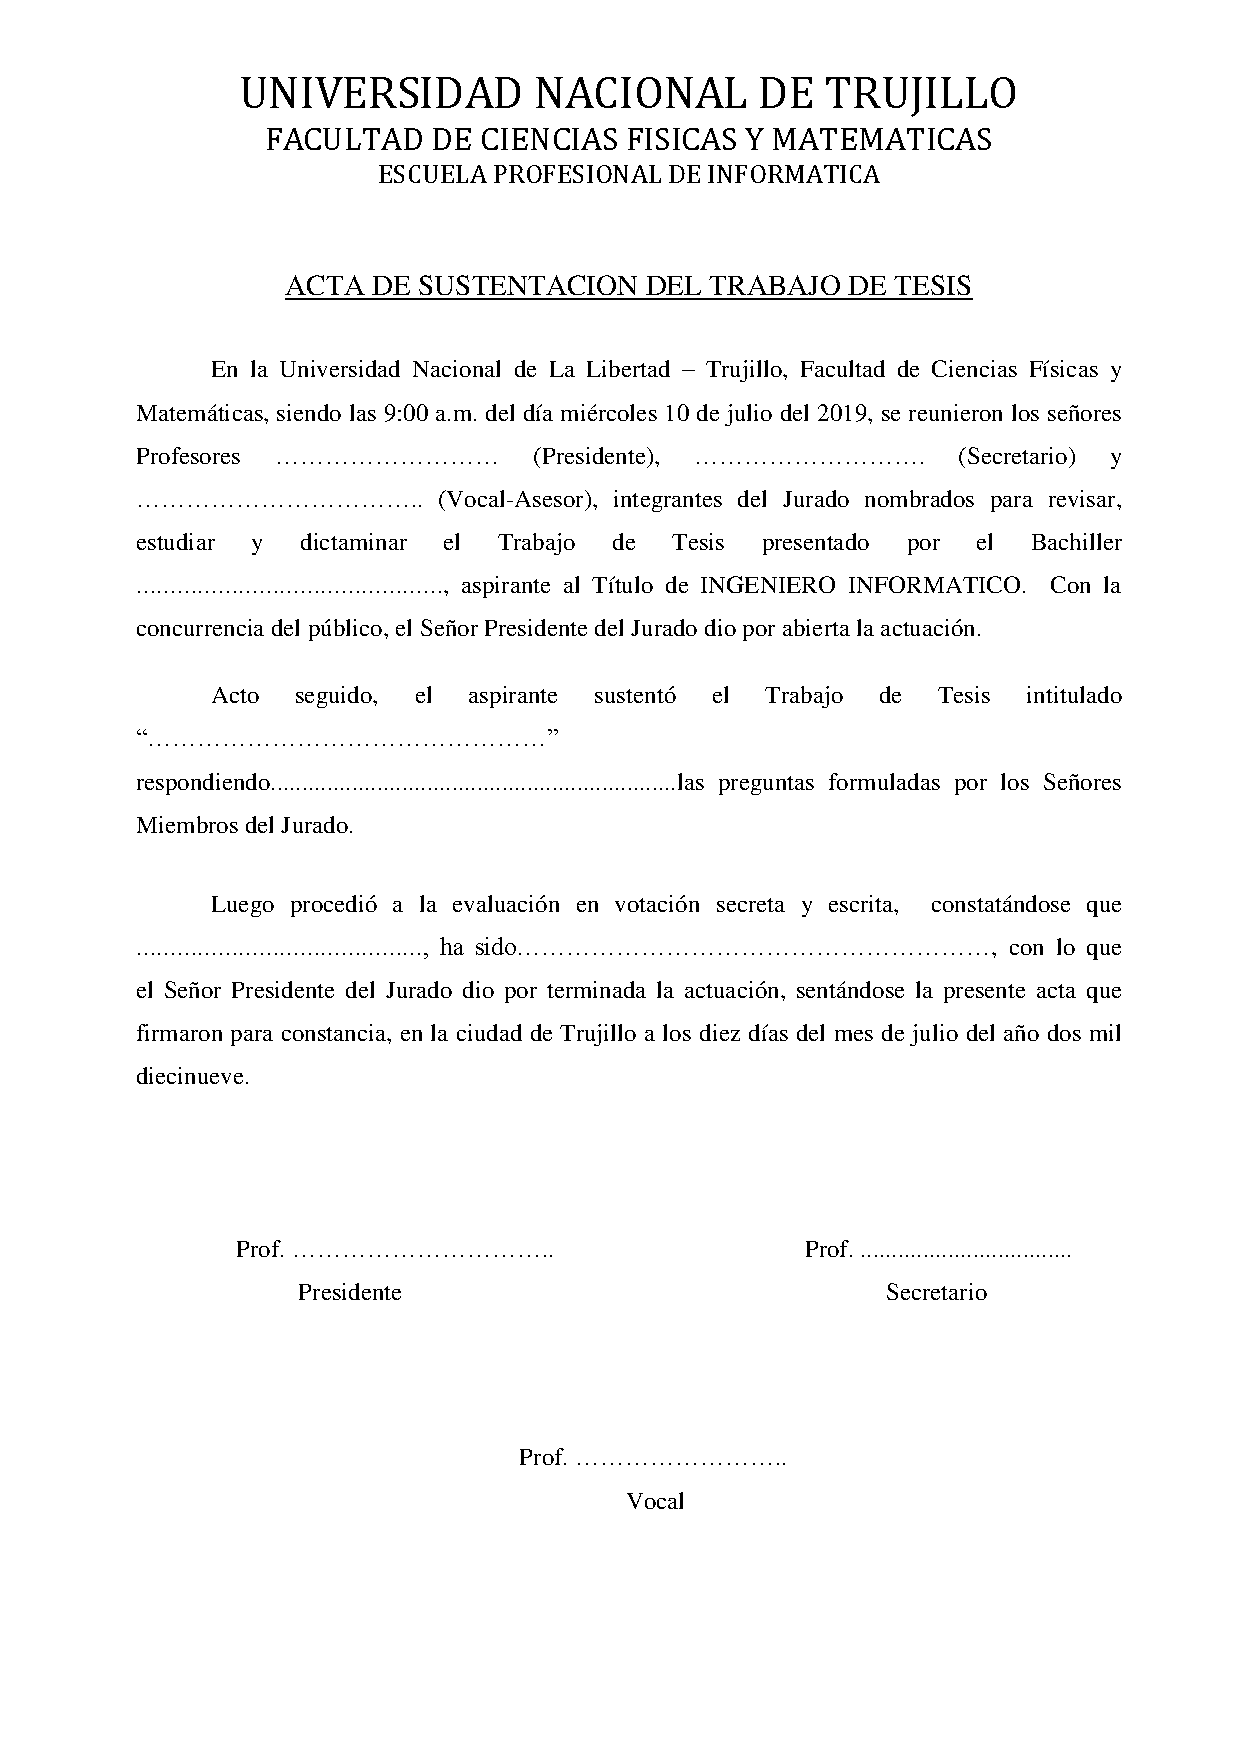
\includepdf[pagecommand={}]{Acta_Sustentacion.pdf}


%%%%%%%%%%%%%%%%%%%%%%%%%%%%%%%%%%%%%%%%%%%%%%%%%%%%%%%%%%%%%%%%%%%

%%%%%%%%%%%%%%%%%%%%%%%%%%%% RESUMEN%%%%%%%%%%%%%%%%%%%%%%
\newpage
\begin{center}
 \addcontentsline{toc}{chapter}{Resumen}
 {\bf\LARGE Resumen}
\end{center} 
\vskip 0.5cm
\begin{quotation}
{\bf Ejemplo:}\par

La investigación bibliográfica revela una preocupación de los gobiernos en lo relacionado al destino final de los residuos sólidos urbanos (RSU), con el objetivo de preservar la salud de la población, el medio ambiente urbano y rural. En este contexto y para el caso de las ciudades peruanas se esperaba que con la desactivación legal de los botaderos hasta el año 2020, surgiesen medidas que viabilicen la colecta selectiva, reciclaje y reutilización para aproximadamente el $80\%$ del volumen total de residuos colectados y destinados a locales no apropiados. 
\vskip 0.2cm 
En este sentido esta investigación tiene como objetivo principal modelar y planificar una red de logística reversa para una región urbana, dimensionando el flujo de RSU que será movido a lo largo de la red, el número y capacidad de las estaciones de colecta, de las unidades productivas y especiales necesarias para su colecta, transporte y disposición final. Los resultados muestran que es posible realizar un modelo matemático para este tipo de problemas, así como su aplicación en diversas regiones sin necesidad de grandes cambios en el modelo propuesto.    

\vskip 0.3cm
\hspace*{-0.6cm}{\bf Palabras claves:} residuos sólidos urbanos, logística reversa, modelo matemático.
\end{quotation}
%%%%%%%%%%%%%%%%%%%%%%%%%%%%%%%%%%%%%%%%%%%%%%%%%%%%%%%%%%%%%%%%%%%%%%%%%%%%%%%%%%%%


%%%%%%%%%%%%%%%%%%%%%%%%%%%%ABSTRACT%%%%%%%%%%%%%%%%%%%%%%
\newpage
\begin{center}
 \addcontentsline{toc}{chapter}{Abstract}
 {\bf\LARGE Abstract}\vskip 1.5cm
\end{center} 
\begin{quotation}

{\bf Ejemplo:}\par

The literature reveals a concern of Governments with the disposal of municipal solid waste (MSW) in order to preserve the health of the population, the urban and rural environment. In this context and for the case of peruvian cities, it was expected that, with the legal command for the deactivation of landfills by 2020, measures would be adopted in order to enable the selective collection, recycling and reuse for about $80\%$ of the total volume of collected solid waste and intended to inappropriate places. 
\vskip 0.2cm
In this sense, this research aims to model and plan a reverse logistics network to an urban area, dimensioning the flow of MSW that will be moved along the network, the number and capacity of collection stations, and the productive and special units required for their collection, transportation and final disposal. The results show to be possible perform mathematical modeling of this problem with low investment, as well as apply it in various regions without major changes in the proposed model.

\vskip 0.3cm
\hspace*{-0.6cm}{\bf Keywords:} solid waste, reverse logistics, mathematical modeling.
\end{quotation}
%%%%%%%%%%%%%%%%%%%%%%%%%%%%%%%%%%%%%%%%%%%%%%%%%%%%%%%%%%%%%%%%%%%%%%%%%%%%%%


%%%%%%%%%%%%%%%%%%%%%%%%%%% LISTA DE SIMBOLOS %%%%%%%%%%%%%%%%%%%%%%
\newpage
\addcontentsline{toc}{chapter}{Lista de símbolos}
 {\bf\LARGE Lista de símbolos}
 \vskip 1.5cm
Constantes: 
\begin{enumerate}
\item[(1)]$r,\overline{r} $ \hspace*{0.8cm} Indice que denota regiones.
\item[(2)] $n $ \hspace*{1.1cm} Indice de bienes finales deseados por los consumidores.
\item[(3)] ...
\vskip 3cm
\end{enumerate} 
\vskip 0.3cm
Variables:
\begin{enumerate}
\item[(5)] $ x^{r} $ \hspace*{1cm} Vector columna que denota la actividad de producción.
\item[(6)] $ u^{r} $ \hspace*{1.2cm} . . .
\end{enumerate}

